%!TEX root = ../main.tex

\chapter{Related Work}

\label{Chapter2-related-work}

\section{Transactional Dataflow Systems}

Transactional dataflow systems are a class of distributed systems designed to handle large-scale data processing with transactional guarantees.
They provide a programming model that allows developers to write declarative, data-driven computations that automatically handle fault tolerance, scalability, and consistency.

Transactional dataflow SFaaS (Stateful Function-as-a-Service) systems are cloud-based systems that provide a serverless platform for processing large-scale data with transactional guarantees.
These systems allow users to write and deploy stateful individual functions or small pieces of code that are triggered in response to events, such as incoming data or scheduled tasks. They are build on top of dataflow systems because they provide fault tolerance, scalability and consistency out-of-the-box.

One of the most prominent transactional dataflow SFaaS system is Apache Flink's [\cite{apache-flink}] StateFun, the architecture of which is shown in figure \ref{fig:statefun-arch} (credited to \cite{transactions-serverless-functions-leveraging-stateful-dataflows}).

\begin{figure}[h]
    \centering
    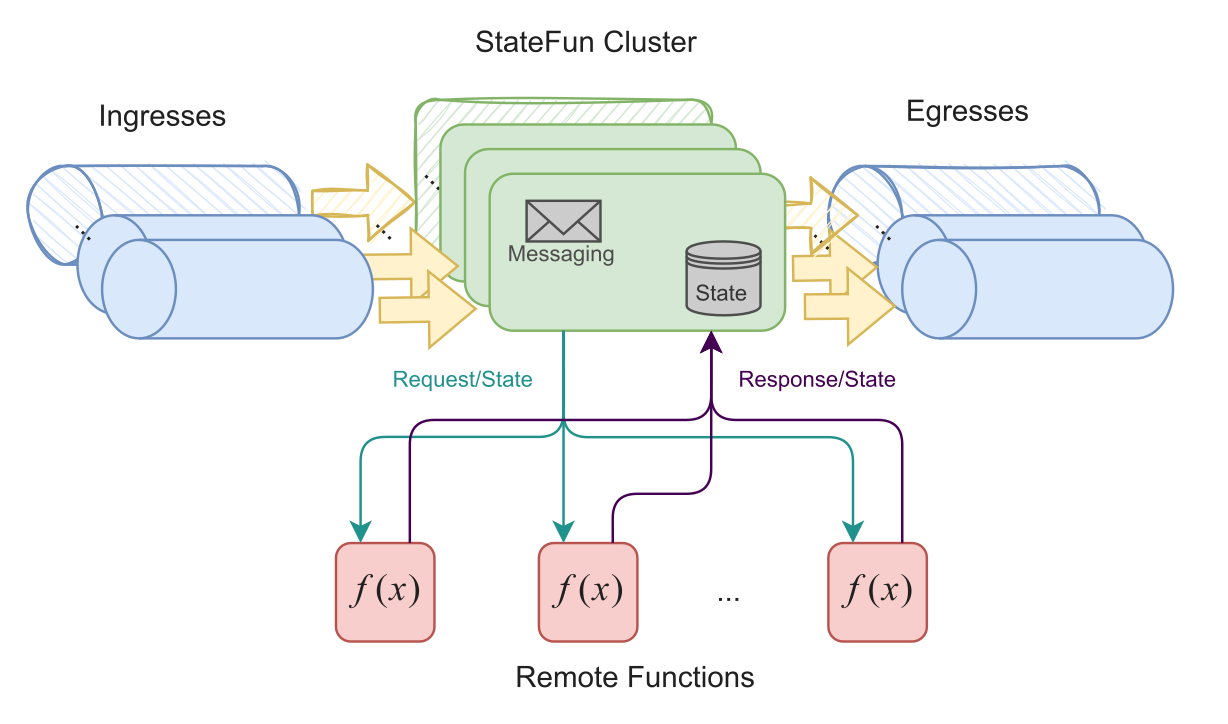
\includegraphics[width=0.8\textwidth]{statefun-arch.png}
    \caption{Architecture of Apache StateFun}
    \label{fig:statefun-arch}
\end{figure}

Remote functions are executed in the nodes of the StateFun cluster, and each node saves its state into an embedded key-value store, as the state can be modelled effectively by a collection of key-value pairs.

In relation to the current work, this is the model architecture for which we will optimize our key-value stores. More concretely, we assume that the key-value stores are to be used as embedded key-value stores in a similar cluster, and that there exists some reliable remote storage in the cloud to store our snapshots.

\section{Key-value stores}

A key-value store is a type of database that uses a simple key-value data model to store data.
In a key-value store, data is represented as a collection of key-value pairs, where each key is a unique identifier that is associated with a corresponding value.

Key-value stores are designed for efficient and fast access to data, making them suitable for use cases where high performance and low latency are critical.

There are various types of key-value stores, each of which is optimized for specific use cases and applications. A fundamental factor that determines the properties of a key-value store is its backend, i.e. the data structures that power it. The main backends for key-value stores are B-Trees, LSM-Trees, and on-disk hash-tables if they store their data on disk, or other tree-based or hash-based data structures if they store their data in memory. Of course, there are also hybrids that combine other types.

\subsection{Types of key-value store backends}

\subsubsection{B-Trees}

A B-tree is a data structure used to store and organize data in a sorted manner, allowing for efficient search, insertion, and deletion operations [\cite{b-tree}]. It is a balanced tree structure, meaning that the height of the tree is kept relatively low compared to the number of elements it contains, which in turn ensures fast access and modification times.

The B-tree consists of nodes, each containing a number of keys and pointers to child nodes. The keys are sorted in ascending order within each node, and the pointers are used to traverse the tree and locate the desired key or node. The number of keys and pointers in each node is fixed, and typically determined by the size of a disk block or page. An example of how key-value lookups work in B-Trees can be found in figure \ref{fig:b-tree}.

\begin{figure}[h]
    \centering
    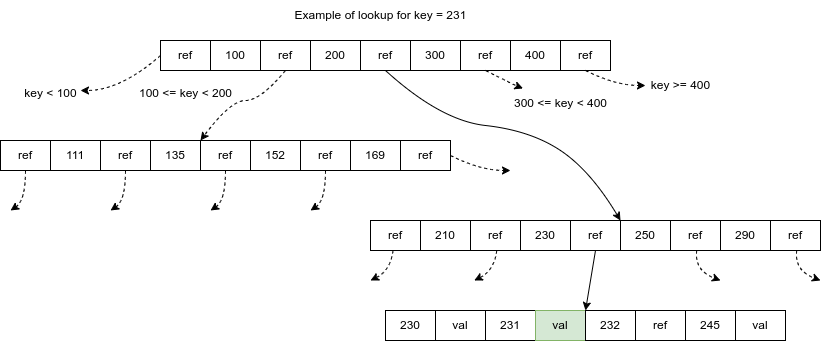
\includegraphics[width=1\textwidth]{b-tree.png}
    \caption{Key lookup example in a B-Tree.}
    \label{fig:b-tree}
\end{figure}

B-trees are commonly used in database systems (especially relational database systems), file systems, and other applications that require fast and efficient access to large amounts of data stored on disk or in memory. However, the B-tree significantly escalates the I/O costs of transactions, as it necessitates real-time maintenance of the index. Consequently, this results in a considerable rise in the overall system cost, reaching up to a fifty percent increase in I/O operations [\cite{lsmtree}].

\subsubsection{Log-Structured Merge-Trees}

The Log-structured Merge-Tree [\cite{lsmtree}] (or LSM-Tree for short) is another popular data-structure used in modern database systems.

At its core, the LSM-tree consists of two main components: a memory component, often called the memtable, that serves as an in-memory buffer and a series of on-disk components, typically referred to as levels. The levels themselves are comprised of immutable SSTables, short for sorted-string tables, or just ``runs''. The writes to the LSM-Tree are flushed directly to disk, and the runs are then merged periodically to garbage-collect overwritten records. The LSM-Trees' internals are analyzed in detail in Chapter \ref{Chapter3-implementation}.

In comparison to the B-Trees, LSM-Trees have several advantages (or trade-offs to be more accurate):

\begin{itemize}
    \item The LSM-trees excel in workloads with heavy write operations (inserts-updates-deletes). Since writes are initially buffered in the memtable and flushed to disk periodically, LSM-trees minimize disk I/O operations, resulting in significantly faster write performance compared to B-trees. B-trees, on the other hand, require immediate disk writes for every update, which can be a performance bottleneck in write-intensive workloads. However, B-Trees typically are more suitable for read-intensive workloads.

    \item LSM-Trees are usually more space-efficient, leading to less disk space usage. B-Trees often suffer from fragmentation, where deleted or updated entries leave behind empty or partially-filled nodes. LSM-trees consolidate data during the compaction process, eliminating duplicates and reclaiming space, leading to improved space utilization. In addition, data is LSM-Trees can be relatively easily compressed, leading to even more efficient space utilization.

    \item In storage systems, a phenomenon known as \textit{write amplification} [\cite{write-amplification,space-amplification}] occurs, which can have a detrimental effect on disk durability and performance, especially in SSD drives. Write amplification refers to the situation where a single database write operation triggers multiple physical writes to the disk. This phenomenon is more pronounced in B-trees in comparison to the LSM-trees, because multiple random page writes are needed to update a single value and the index. LSM-Trees are less susceptible to this phenomenon because they write data sequentially, leading to less susceptibility to write amplification. Sequential writes also lead to a performance boost, especially in rotational HDD disks.

    \item Due to the way LSM-Trees organize their data immutably into levels, they allow for fast recovery, and most importantly for efficient incremental snapshots. \textit{All the recent writes are located in higher levels of the LSM-Tree and therefore when taking a snapshot we can exclude the lower levels if they have been included in a previous snapshot}. With a B-Tree, incremental snapshots would be challenging to achieve because of their in-place updates. We would need to maintain additional data-structures to keep track of what exactly was changed, and make these data-structures persistent as well.
\end{itemize}

While log-structured storage offers numerous benefits, it does have a drawback related to the compaction process, which can occasionally impact the performance of concurrent read and write operations. As disks have limited bandwidth, allocating a significant portion of it to merging operations can adversely affect data writes. This can result in a slight reduction in throughput and average response time. The impact is typically minimal but in certain cases, particularly at higher percentiles, queries to log-structured storage engines may experience relatively high response times. In such scenarios, B-trees tend to offer more predictable and consistent performance.

Additionally, in B-trees each key exists in precisely one location within the index, unlike log-structured storage engines where multiple copies of the same key may reside in different segments. This characteristic makes B-trees appealing in databases that aim to provide robust transactional semantics. Many relational databases, for instance, implement transaction isolation by applying locks to key ranges. In a B-tree index, these locks can be directly associated with the tree, making it easier to manage and enforce transactional consistency. For our use case, this characteristic is not important, because all transactional logic is handled at higher levels by the transactional dataflow system.

\subsubsection{Fractal Trees}

Fractal Trees are a type of indexing data structure that are designed to provide high performance and scalability in multi-core environments. They are primarily based on B-Trees.

The key idea behind Fractal Trees is to split the index into a set of smaller indexes, each of which is optimized for a specific data access pattern. This allows the system to scale horizontally across multiple cores and nodes, while also providing high performance for a wide range of workloads.

Like B-Trees, there are good for transactions at the database level, because each key exists in only one copy in the tree. Compared to LSM-Trees, they can offer some advantage in terms of mitigating write amplification [\cite{fractal-trees}], but the advantage is insignificant in leveled many-runs-per-level LSM-Trees (which is the kind of LSM-Tree presented and implemented in Chapter \ref{Chapter3-implementation}).

\subsubsection{On-disk hash-tables}

On-disk hash-tables, also known as persistent hash-tables, are data structures that allow efficient storage and retrieval of key-value pairs on disk. On-disk hash-tables use hashing algorithms to map keys to specific locations on the disk, enabling fast retrieval of values associated with the keys. The hash-table is typically divided into fixed-size buckets or blocks, each containing a certain number of key-value pairs. One prominent example of a database that uses on-disk hash-tables is the \cite{gdbm} project.

\subsubsection{In-memory key-value stores}

In-memory key-value stores, as the name implies, store and retrieve data entirely in main memory, providing fast and efficient access to key-value pairs. Unlike disk-based storage systems, which store data on hard drives, in-memory key-value stores keep the entire dataset in RAM, eliminating the latency associated with disk I/O operations, allowing for extremely low access times, making them ideal for applications that require high-performance data retrieval, such as caching, real-time analytics, and session management. However, the limited capacity of RAM restricts the size of the dataset that can be stored in-memory, making these stores more suitable for smaller to moderate-sized datasets that can fit within the available memory. A well-known commercial in-memory key-value store is \cite{redis}.

\subsubsection{Hybrids}

There are databases that leverage more than one data structure to store and retrieve data. Microsoft's \textsc{Faster} \cite{faster} for instance uses in-memory components with log-structured on-disk storage to combine the best between two worlds. We analyze \textsc{Faster} in detail in chapter \ref{Chapter3-implementation}, as it is one of the implemented stores.

\subsection{Key-value stores in dataflow systems}

The most prominent key-value store used as embedded key-value store in distributed streaming/dataflow systems is \cite{rocksdb}, an LSM-Tree-based store. It is used in Apache Spark Structured Streaming [\cite{spark-steaming}], Apache Flink [\cite{apache-flink}], \cite{kafka} and Apache Samza [\cite{samza}]. In the work of \cite{workload-aware-streaming-state-management}, the authors have also integrated \textsc{Faster} in a dataflow system seamlessly.

\section{Incremental Snapshots}

Snapshots play a vital role in distributed systems, as they enable the creation of a consistent snapshot representing the global state of the system. However, achieving this consistency is challenging due to the absence of globally shared memory and a synchronized global clock.

Extensive research has been conducted on snapshotting algorithms, as documented in literature such as the work by \cite{snapshots-rollbacks}. While these algorithms have received significant attention, there has been limited exploration of efficient incremental snapshots, which aim to leverage previous snapshots to avoid redundant work.

The problem of incremental snapshots can be seen as an extension of the broader challenge of distributed state synchronization, which focuses on maintaining consistency across distributed systems. In the next sections we present the approach of some commercial systems to this problem, as well as some data structures commonly used for state synchronization.

\subsection{Incremental Snapshots in Distributed Systems}

Apache Flink [\cite{apache-flink}] leverages the properties of the log-structured storage and the concept of \textit{delta maps} (see section \ref{data-structs-sync}) [\cite{state-management-apache-flink}] for incremental snapshots, although as for the time this related work was published, it hasn't been implemented. This approach is the one we generally follow in implementing the incremental snapshotting functionality in the key-value stores in Chapter \ref{Chapter3-implementation}.

In the work of \cite{fraser-diff-sync}, the author introduces the concept of \textit{Differential Synchronization} for synchronizing changes to a single document edited by multiple users in parallel. The approach is interesting but too high-level for our use-case.

\subsection{Data structures for efficient state synchronization}
\label{data-structs-sync}

Low-level synchronization mechanisms usually make use of specific data structures. In the following subsections, we examine three of the most prominent ones.

\subsubsection{Delta maps}

A delta map is a data structure or mechanism used to track and represent changes or differences between two versions of a dataset or state. It provides a way to efficiently transmit and apply updates across distributed nodes without transferring the entire dataset.

Delta maps are usually implemented with version vectors or logs, depending on the problem and the application. The synchronization approach with delta maps using version vectors is more carefully examined in Chapter \ref{Chapter3-implementation} because it is the approach we will use ourselves for detecting the changes needed to be synchronized between the key-value stores and remote object storage systems.

\subsubsection{Merkle trees}

Merkle trees [\cite{merkle-trees}] are a cryptographic data structure that facilitate efficient and secure verification of data integrity. They operate by organizing data into a tree-like structure, where each leaf node represents a small portion of data and the intermediate nodes store the hash values of their child nodes. The process of constructing a Merkle tree involves recursively hashing pairs of nodes until a single root hash, called the Merkle root. This root hash serves as a compact representation of the entire data set, allowing for efficient lookup of changes. An example of a Merkle-Tree is shown in figure \ref{fig:merkle-tree} \footnote{Credits to Wikipedia}.

\begin{figure}[h]
    \centering
    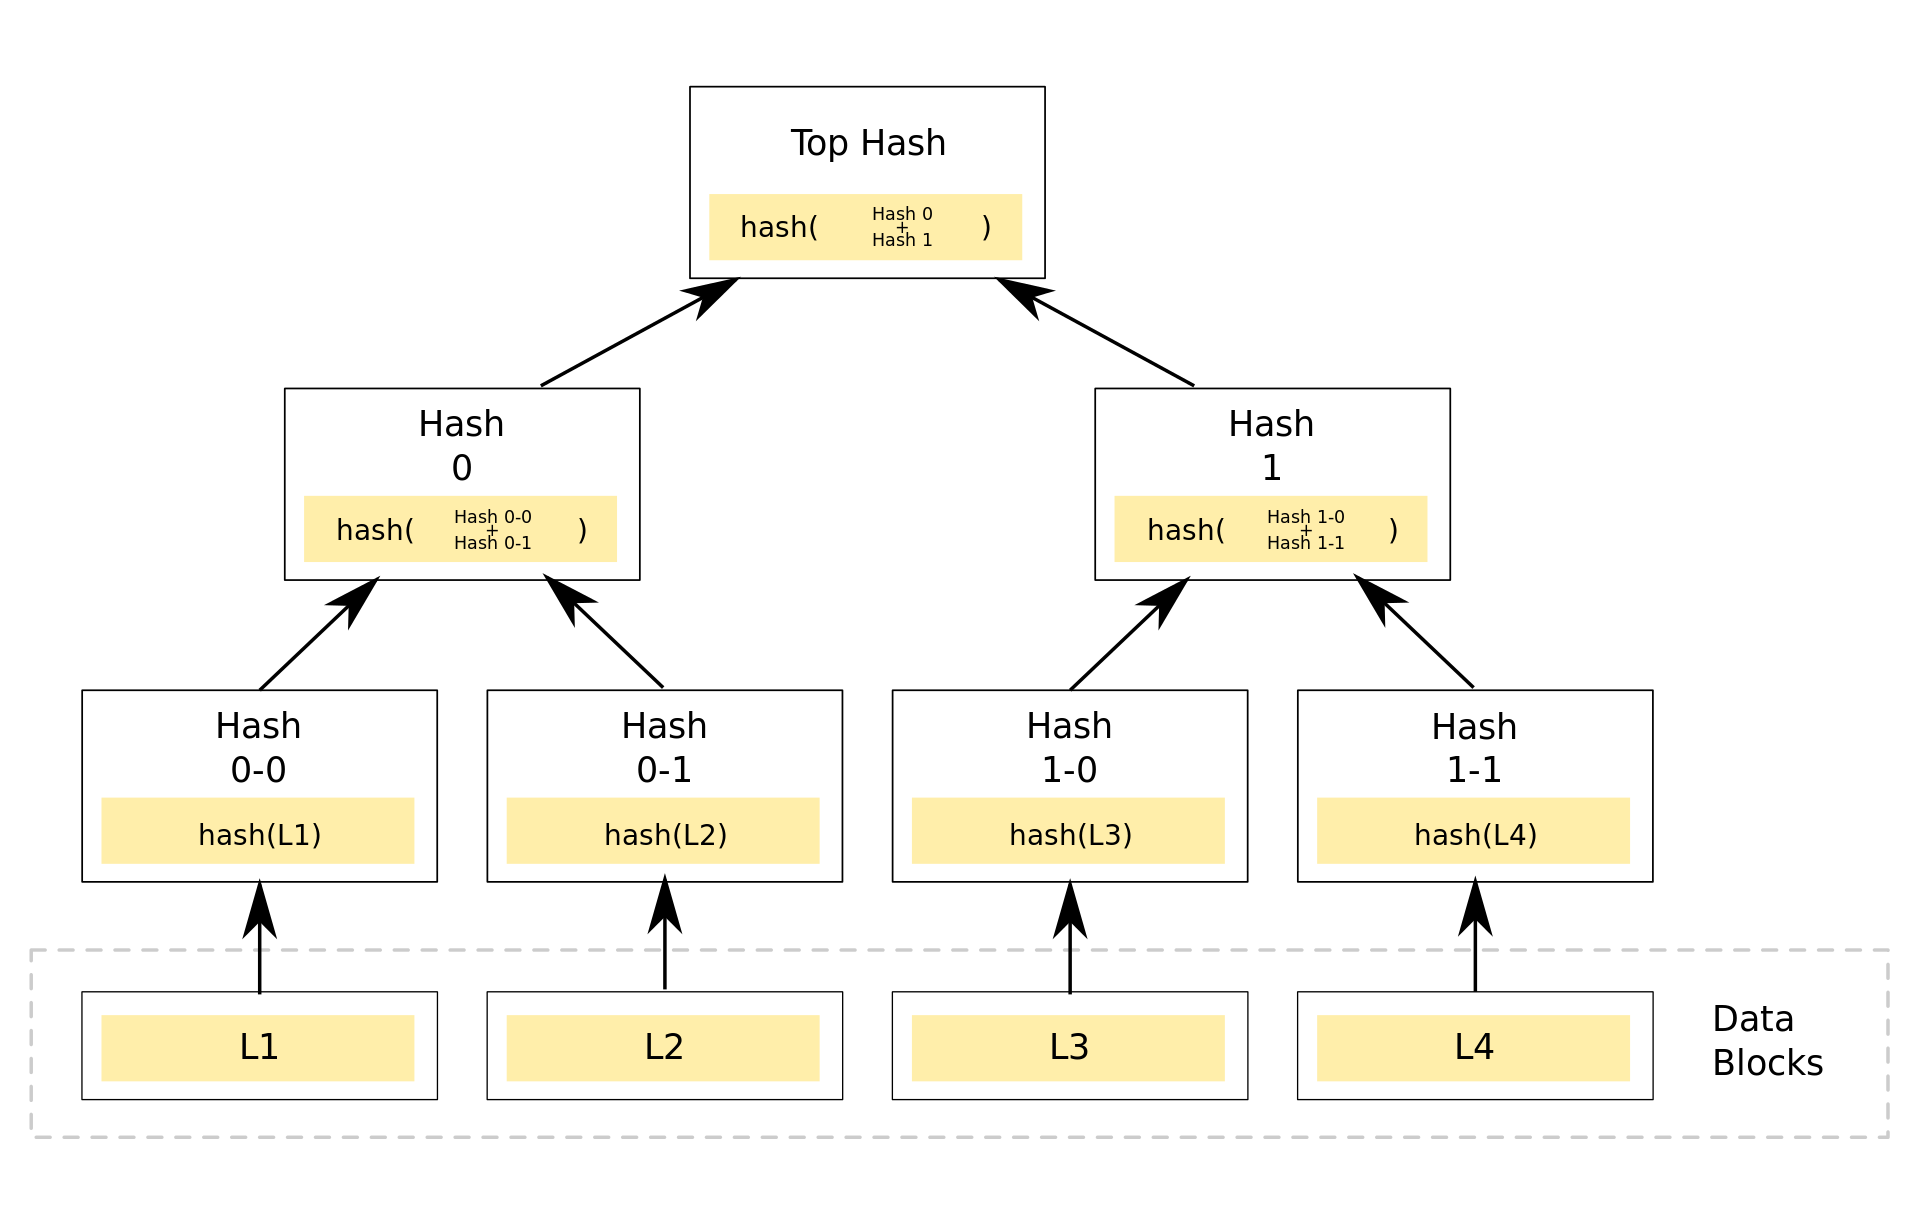
\includegraphics[width=1\textwidth]{merkle-tree.png}
    \caption{Example of a simple Merkle Tree.}
    \label{fig:merkle-tree}
\end{figure}

In the context of synchronizing distributed systems, Merkle trees play a crucial role. They enable multiple parties to compare and synchronize their datasets by efficiently identifying differences in data without transferring the complete dataset. By comparing the Merkle root hashes, participants can determine if their datasets are identical or if specific portions of the data have diverged. This approach minimizes the amount of data that need to be exchanged and reconciled, reducing bandwidth requirements and synchronization time.

\subsubsection{Conflict-Free Replicated Data Types (CRDTs)}

Related to the field of replica-synchronization, especially in implementing \textit{eventual consistency} in distributed systems is the concept of Conflict-Free Replicated Data Types (or CRDTs) [\cite{crdts}].

CRDTs are a class of data structures designed for distributed systems that aim to provide strong eventual consistency without the need for coordination or centralized authority. They are specifically designed to handle concurrent updates in a distributed environment where there may be latency, network partitions, or conflicting operations.

The key idea behind CRDTs is that they ensure convergence by allowing updates to be commutative and/or associative, meaning that the order of concurrent operations does not affect the final state of the data.

CRDTs have been implemented for a variety of lower-level data structures like counters, sets, maps, registers, even JSONs [\cite{json-crdt}].
